\documentclass{beamer}\usepackage[]{graphicx}\usepackage[]{color}
% maxwidth is the original width if it is less than linewidth
% otherwise use linewidth (to make sure the graphics do not exceed the margin)
\makeatletter
\def\maxwidth{ %
  \ifdim\Gin@nat@width>\linewidth
    \linewidth
  \else
    \Gin@nat@width
  \fi
}
\makeatother

\definecolor{fgcolor}{rgb}{1, 0.894, 0.769}
\newcommand{\hlnum}[1]{\textcolor[rgb]{0.824,0.412,0.118}{#1}}%
\newcommand{\hlstr}[1]{\textcolor[rgb]{1,0.894,0.71}{#1}}%
\newcommand{\hlcom}[1]{\textcolor[rgb]{0.824,0.706,0.549}{#1}}%
\newcommand{\hlopt}[1]{\textcolor[rgb]{1,0.894,0.769}{#1}}%
\newcommand{\hlstd}[1]{\textcolor[rgb]{1,0.894,0.769}{#1}}%
\newcommand{\hlkwa}[1]{\textcolor[rgb]{0.941,0.902,0.549}{#1}}%
\newcommand{\hlkwb}[1]{\textcolor[rgb]{0.804,0.776,0.451}{#1}}%
\newcommand{\hlkwc}[1]{\textcolor[rgb]{0.78,0.941,0.545}{#1}}%
\newcommand{\hlkwd}[1]{\textcolor[rgb]{1,0.78,0.769}{#1}}%
\let\hlipl\hlkwb

\usepackage{framed}
\makeatletter
\newenvironment{kframe}{%
 \def\at@end@of@kframe{}%
 \ifinner\ifhmode%
  \def\at@end@of@kframe{\end{minipage}}%
  \begin{minipage}{\columnwidth}%
 \fi\fi%
 \def\FrameCommand##1{\hskip\@totalleftmargin \hskip-\fboxsep
 \colorbox{shadecolor}{##1}\hskip-\fboxsep
     % There is no \\@totalrightmargin, so:
     \hskip-\linewidth \hskip-\@totalleftmargin \hskip\columnwidth}%
 \MakeFramed {\advance\hsize-\width
   \@totalleftmargin\z@ \linewidth\hsize
   \@setminipage}}%
 {\par\unskip\endMakeFramed%
 \at@end@of@kframe}
\makeatother

\definecolor{shadecolor}{rgb}{.97, .97, .97}
\definecolor{messagecolor}{rgb}{0, 0, 0}
\definecolor{warningcolor}{rgb}{1, 0, 1}
\definecolor{errorcolor}{rgb}{1, 0, 0}
\newenvironment{knitrout}{}{} % an empty environment to be redefined in TeX

\usepackage{alltt}
\usepackage{../371g-slides}
\title{Review of Inference}
\subtitle{Lecture 8}
\author{STA 371G}
\IfFileExists{upquote.sty}{\usepackage{upquote}}{}
\begin{document}
  
  

  \frame{\maketitle}

  % Show outline at beginning of each section
  \AtBeginSection[]{
    \begin{frame}<beamer>
      \tableofcontents[currentsection]
    \end{frame}
  }

  %%%%%%% Slides start here %%%%%%%

  \begin{darkframes}
    \begin{frame}{Updated schedule}
      \begin{itemize}
        \item Nothing due this week!
        \item Quiz 3 next Tuesday
        \item No Quiz 4
        \item HW 3 \& 4 due due next Monday
        \item See updated syllabus on Canvas for all details
      \end{itemize}
    \end{frame}

    \begin{frame}{About the project}
      \begin{itemize}[<+->]
        \item Build a regression model to answer a research question that is of interest to you, using either the GSS (General Social Survey) or Add Health (National Longitudinal Study of Adolescent to Adult Health) data set
        \item You pick your research question (e.g. predict how much people drink based on their drinking history, personal characteristics, and mental health history)
        \item You cannot use the same research question as another group
        \item You'll be assigned to a group, but can choose to work alone (let me know by EOD \alert{tomorrow} if you want to work alone)
        \item The project is divided into multiple components; you'll write a group paper in phases over the remainder of the semester
      \end{itemize}
    \end{frame}

    \begin{frame}{Project components}
      \begin{itemize}
        \item March 11: Initial proposal (5\%)
        \item March 25: Literature review (10\%)
        \item April 1: Final proposal (5\%)
        \item April 15: Exploratory data analysis (10\%)
        \item April 29: Final paper submission (60\%)
        \item May 3, 5, 18: Presentation \& peer evaluations (10\%)
      \end{itemize}
    \end{frame}

    \begin{frame}{Review of Inference}
      \begin{itemize}
        \item Today we'll review key terms around statistical inference: hypothesis tests, confidence intervals, and $p$-values
        \item We'll also touch on how to run simulations in R (which we unfortunately had to cut from the curriculum due to the UT closure)
        \item The concepts are the most important; the specific details of the applications here are not critical
      \end{itemize}
    \end{frame}

    \section{Minecraft speedrunning controversy}

    \begin{frame}{Minecraft video game speedrunning}
      \begin{itemize}[<+->]
        \item ``Speedrunning'' in video games is the process of trying to beat video games as fast as possible (e.g., the current world record for Super Mario Bros on Nintendo is under 5 min!)
        \item Speedruns are often streamed on YouTube or Twitch and can be big business!
        \item One Minecraft speedrunner, ``Dream,'' has 18M subscribers and 1.5B views on YouTube, which could result in millions of dollars in ad revenue
        \item But Dream was suspected of cheating---how can you prove it?
      \end{itemize}
    \end{frame}

    \begin{frame}{How Minecraft works (sort of)}
      \begin{columns}
        \begin{column}{0.5\textwidth}
          \begin{itemize}[<+->]
            \item To beat the game, you need 12 ``eyes of ender''
            \item You can obtain an eye of ender by trading for a pearl, plus some ``blaze powder''
            \item Every time you attempt a trade, there is a 4.73\% chance you will get a pearl
            \item As a result, luck plays a big factor in how quickly you can beat the game
          \end{itemize}
        \end{column}
        \begin{column}{0.5\textwidth}
          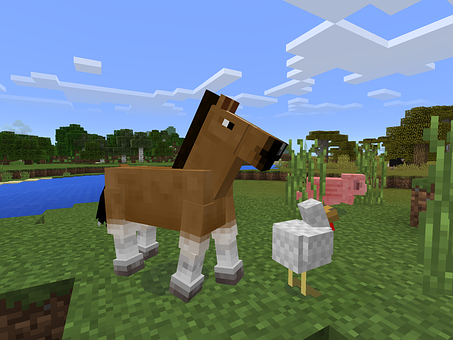
\includegraphics[width=\textwidth]{minecraft}
        \end{column}
      \end{columns}
    \end{frame}

    \begin{frame}[fragile]{Dream's luck}
      \begin{itemize}[<+->]
        \item The specific calculations here aren't important, but let's get a number anyway
        \item Dream attempted 262 trades, and got pearls in 42 of them (16\%)---much higher than the 4.73\% expected by chance
        \item Assuming no cheating, the number of pearls obtained in 262 trials is Binomial ($n=262$, $p=0.0473$)
        \item We can calculate the chance of having luck this good ($P(\text{number of pearls} \geq 42)$) with R:
      \end{itemize}
      \pause
\begin{knitrout}
\definecolor{shadecolor}{rgb}{0.137, 0.137, 0.137}\color{fgcolor}\begin{kframe}
\begin{alltt}
\hlnum{1} \hlopt{-} \hlkwd{pbinom}\hlstd{(}\hlnum{41}\hlstd{,} \hlnum{262}\hlstd{,} \hlnum{0.0473}\hlstd{)}
\end{alltt}
\begin{verbatim}
[1] 5.65e-12
\end{verbatim}
\end{kframe}
\end{knitrout}
    \end{frame}

    \begin{frame}{Dream's luck}
      \begin{itemize}[<+->]
        \item In other words, \emph{for someone that is not cheating}, there is about a 1 in 177 billion chance of having luck as good or better than Dream claimed to.
        \item This indicates that Dream's claim is implausible (10 runs an hour, 24 hours/day, for 100 years, is just 8.8 million attempts)
        \item In other words, we can be confident that Dream was cheating
      \end{itemize}
    \end{frame}

    \begin{frame}{Restating this formally}
      \begin{itemize}[<+->]
        \item The \alert{null hypothesis} ($H_0$) is what we assume to be true in the absence of evidence to the contrary: \alert{Dream is not cheating}
        \item The \alert{alternative hypothesis} ($H_A$) is what we will believe if it turns out that $H_0$ is false: \alert{Dream is cheating}
        \item The $p$-value is the conditional probability of seeing data at least as extreme as what was observed, given that $H_0$ is true: \alert{$p=\text{1 in 177 billion}$}
        \item If $p$ is small, we will reject $H_0$ and believe $H_A$. Otherwise, we continue to believe $H_0$: \alert{reject $H_0$}
      \end{itemize}
    \end{frame}

    \section{Sampling distributions and $t$-tests}

    \begin{frame}[fragile]{GPAs of all UT students entering in Fall 2000}
\begin{knitrout}
\definecolor{shadecolor}{rgb}{0.137, 0.137, 0.137}\color{fgcolor}
\includegraphics[width=\maxwidth]{/tmp/figures/unnamed-chunk-3-1} 

\end{knitrout}
    \end{frame}
      
      
    \begin{frame}[fragile]{Let's take a sample}
      Usually, we only have access to a sample of the data. Let's pretend that we only had a sample of $n=100$ students:
\begin{knitrout}
\definecolor{shadecolor}{rgb}{0.137, 0.137, 0.137}\color{fgcolor}\begin{kframe}
\begin{alltt}
\hlstd{sample.gpas} \hlkwb{<-} \hlkwd{sample}\hlstd{(ut2000}\hlopt{$}\hlstd{GPA,} \hlnum{100}\hlstd{)}
\hlkwd{mean}\hlstd{(sample.gpas)}
\end{alltt}
\begin{verbatim}
[1] 3.2
\end{verbatim}
\end{kframe}
\end{knitrout}
      Since we have a random sample, it's a good, but not perfect, estimate of the population GPA (3.212). \pause But normally we don't have access to the population, so we don't know how good our estimate is!
    \end{frame}
      
    \begin{frame}
      \begin{center}
        Normally we only have access to one sample. 
        
        \pause\vspace{2em}
        Since we have the population, we can \alert{simulate} what would happen if we repeatedly took samples over and over from the same population.
      \end{center}
    \end{frame}  

    \begin{frame}[fragile]
\begin{knitrout}
\definecolor{shadecolor}{rgb}{0.137, 0.137, 0.137}\color{fgcolor}\begin{kframe}
\begin{alltt}
\hlstd{sample.means} \hlkwb{<-} \hlkwd{replicate}\hlstd{(}\hlnum{10000}\hlstd{, \{}
  \hlstd{the.sample} \hlkwb{<-} \hlkwd{sample}\hlstd{(ut2000}\hlopt{$}\hlstd{GPA,} \hlnum{100}\hlstd{)}
  \hlkwd{return}\hlstd{(}\hlkwd{mean}\hlstd{(the.sample))}
\hlstd{\})}
\hlkwd{hist}\hlstd{(sample.means,} \hlkwc{main}\hlstd{=}\hlstr{""}\hlstd{,} \hlkwc{col}\hlstd{=}\hlstr{"orange"}\hlstd{)}
\end{alltt}
\end{kframe}
\includegraphics[width=\maxwidth]{/tmp/figures/unnamed-chunk-5-1} 

\end{knitrout}
    \end{frame}
      
      
    \begin{frame}[fragile]{Sampling distribution of $\overline{GPA}$}
      The \emph{sampling distribution} of $\overline{GPA}$ is the distribution of sample means, if we took an infinite number of repeated samples:      
      \begin{align*}
        E(\overline{GPA}) &= \mu = 3.212 \\
        \text{SD}(\overline{GPA}) &= \frac{\sigma}{\sqrt n} = \frac{0.48}{\sqrt{100}} = 0.048
      \end{align*}
      
      The last value quantifies how much the sample mean will vary from sample to sample. But we normally can't compute $\sigma$ since we don't have the whole population, so we estimate it by calculating the SD in the \emph{sample} ($\hat\sigma$) and dividing by $\sqrt n$; this is the \emph{standard error of the mean}.
    \end{frame}
      
      
    \begin{frame}{Confidence intervals}
      Given a sample mean, we want to calculate a \emph{confidence interval}, which gives a plausible range of values for the population mean.
      \pause\vspace{2em}
      
      A confidence interval is always of the form
      \[
        \text{sample statistic} \pm (\text{critical value})(\text{standard error}).
      \]
      \pause
      Our sample statistic is $\hat\mu$ and our standard error is $\hat\sigma/\sqrt n$.
      \pause
      What is the critical value?
    \end{frame}
      
      
    \begin{frame}
      As it turns out, the sampling distribution (of $\hat\mu$) is not \emph{quite} Normal. If we standardize the sample means, the distribution of \[ \frac{\hat\mu - \mu}{ \hat\sigma/\sqrt n } \] is called a $t$-distribution with $n-1$ degrees of freedom. \pause The critical value for a 95\% confidence interval is $t^*=\pm1.984$, the value that cuts off 95\% of the area under the $t$-distribution:
      
\begin{knitrout}
\definecolor{shadecolor}{rgb}{0.137, 0.137, 0.137}\color{fgcolor}
\includegraphics[width=\maxwidth]{/tmp/figures/unnamed-chunk-6-1} 

\end{knitrout}
    \end{frame}
      
      
    \begin{frame}[fragile]
      There are two helpful R functions for calculating values around $t$-distributions (like \verb|pnorm| and \verb|qnorm|):
      \begin{itemize}[<+->]
        \item \verb|pt(x, df)| calculates $P(t<x)$ if we are looking at a distribution with $df$ degrees of freedom. \pause
        \item \verb|qt(y, df)| does the opposite; it figures out what value of $x$ will give $P(t<x)=y$. \pause
      \end{itemize}
      So the critical value for a 95\% confidence interval is \verb|qt(.975, 99)| when $n=100$. \pause\bigskip      
    \end{frame}
      
    \begin{frame}
      Using our sample of $n=100$, we calculate that a 95\% confidence interval for the mean population GPA is
      \[
        \hat\mu \pm t^* \frac{\hat\sigma}{\sqrt n}
        \pause\quad\Longrightarrow\quad
        3.204 \pm 1.984\cdot\frac{0.478}{\sqrt{100}}
        \pause\quad\Longrightarrow\quad
        (3.109, 3.299)
      \]
      \pause
      There are two ways to interpret this:
      \begin{itemize}
        \item \textbf{Informally,} we are 95\% confident that the population mean GPA is between 3.109 and 3.299. \pause
        \item \textbf{Formally,} if we took repeated samples and found the 95\% CI within each sample, 95\% of the CIs would contain the population mean.
      \end{itemize}
    \end{frame}
      
      
    \begin{frame}[fragile]
      R can do this work for you!
\begin{knitrout}
\definecolor{shadecolor}{rgb}{0.137, 0.137, 0.137}\color{fgcolor}\begin{kframe}
\begin{alltt}
\hlkwd{t.test}\hlstd{(sample.gpas)}
\end{alltt}
\begin{verbatim}

	One Sample t-test

data:  sample.gpas
t = 67, df = 99, p-value <2e-16
alternative hypothesis: true mean is not equal to 0
95 percent confidence interval:
 3.11 3.30
sample estimates:
mean of x 
      3.2 
\end{verbatim}
\end{kframe}
\end{knitrout}
    \end{frame}
      
      
    \begin{frame}{Hypothesis tests}
      \begin{itemize}[<+->]
        \item Let's say Mr. Sooner comes along and claims that the average UT GPA is actually 3.15.
        \item Let's pretend we don't have the population (which is usually the case), and so we can't know for sure that he is wrong.
        \item We do have some evidence (our sample) that we can bring to bear on the question.
      \end{itemize}
    \end{frame}

    \begin{frame}{Restating this formally}
      \begin{itemize}[<+->]
        \item The \alert{null hypothesis} ($H_0$) is what we assume to be true in the absence of evidence to the contrary: \alert{$\mu=3.15$}
        \item The \alert{alternative hypothesis} ($H_A$) is what we will believe if it turns out that $H_0$ is false: \alert{$\mu\neq 3.15$}
        \item The $p$-value is the conditional probability of seeing data at least as extreme as what was observed, given that $H_0$ is true: \alert{if Sooner is correct, how likely is it that in our sample we would see a sample mean (of $\hat\mu=3.204$) that is so far away from his hypothesized value of $\mu=3.15$?}
      \end{itemize}
    \end{frame}
      
    
      
    \begin{frame}[fragile]
      R can run hypothesis tests for us:
\begin{knitrout}
\definecolor{shadecolor}{rgb}{0.137, 0.137, 0.137}\color{fgcolor}\begin{kframe}
\begin{alltt}
\hlkwd{t.test}\hlstd{(sample.gpas,} \hlkwc{mu}\hlstd{=}\hlnum{3.15}\hlstd{)}
\end{alltt}
\begin{verbatim}

	One Sample t-test

data:  sample.gpas
t = 1, df = 99, p-value = 0.3
alternative hypothesis: true mean is not equal to 3.15
95 percent confidence interval:
 3.11 3.30
sample estimates:
mean of x 
      3.2 
\end{verbatim}
\end{kframe}
\end{knitrout}
    \end{frame}

    \begin{frame}{Restating this formally}
      \begin{itemize}
        \item The \alert{null hypothesis} ($H_0$) is what we assume to be true in the absence of evidence to the contrary: \alert{$\mu=3.15$}
        \item The \alert{alternative hypothesis} ($H_A$) is what we will believe if it turns out that $H_0$ is false: \alert{$\mu\neq 3.15$}
        \item The $p$-value is the conditional probability of seeing data at least as extreme as what was observed, given that $H_0$ is true: \alert{$p=0.3$}
        \item If $p$ is small, we will reject $H_0$ and believe $H_A$. Otherwise, we continue to believe $H_0$: \alert{do not reject $H_0$; Mr Sooner's claim is consistent with our sample data}
      \end{itemize}
    \end{frame}
      
    \begin{frame}
     
      When doing hypothesis testing, we select an $\alpha$ value in advance, and then reject the null hypothesis if and only if $p<\alpha$.
      \pause\bigskip
      
      $\alpha=.05$ is a good ``default'' to use unless you have a reason to set it higher or lower.
    \end{frame}

    \section{Using resampling to conduct hypothesis tests}

    \begin{frame}{Comparing meeting strategies}
      \begin{itemize}
        \item Renuka holds daily ``standup'' meetings with her team, under the theory that having the meeting standing up will make it go faster.
        \item She decides to test this by holding 20 meetings standing up and then 20 meetings sitting down.
        \item Standing is 3.65 minutes faster, but is that real or just due to random chance?
      \end{itemize}
      \begin{center}
        \begin{tabular}{p{2in}p{2in}}
          Standing & Sitting \\
          \hline
          27, 29, 30, 30, 31, 31, 31, 32, 33, 33, 33, 34, 34, 35, 35, 35, 36, 37, 37, 40 &
          30, 33, 34, 34, 34, 34, 35, 35, 36, 36, 37, 38, 38, 38, 39, 39, 40, 40, 41, 45 \\
        \end{tabular}
      \end{center}
    \end{frame}

    \begin{frame}{Resampling strategy}
      \begin{itemize}
        \item Put all 40 meeting times in a blender, and randomly pick out 20 for each group.
        \item Calculate how often do we get a difference by chance of at least 3.65 minutes?
      \end{itemize}
    \end{frame}

    \begin{frame}[fragile]

\begin{knitrout}
\definecolor{shadecolor}{rgb}{0.137, 0.137, 0.137}\color{fgcolor}\begin{kframe}
\begin{alltt}
\hlstd{diffs} \hlkwb{<-} \hlkwd{replicate}\hlstd{(}\hlnum{10000}\hlstd{, \{}
  \hlstd{reordered} \hlkwb{<-} \hlkwd{sample}\hlstd{(}\hlkwd{c}\hlstd{(standing, sitting),} \hlnum{40}\hlstd{)}
  \hlstd{group1} \hlkwb{<-} \hlstd{reordered[}\hlnum{1}\hlopt{:}\hlnum{20}\hlstd{]}
  \hlstd{group2} \hlkwb{<-} \hlstd{reordered[}\hlnum{21}\hlopt{:}\hlnum{40}\hlstd{]}
  \hlkwd{return}\hlstd{(}\hlkwd{mean}\hlstd{(group1)} \hlopt{-} \hlkwd{mean}\hlstd{(group2))}
\hlstd{\})}
\hlkwd{hist}\hlstd{(diffs)}
\end{alltt}
\end{kframe}
\includegraphics[width=\maxwidth]{/tmp/figures/unnamed-chunk-10-1} 

\end{knitrout}
    \end{frame}

    \begin{frame}[fragile]
      Just by looking at the histogram, we can tell 3.65 is a very unusual difference to see just by chance. So the $p$-value is low and we should reject the null hypothesis.

      \pause
      \vspace{2em}

      To calculate it exactly, we count the number of differences that are larger than $\pm 3.65$:
\begin{knitrout}
\definecolor{shadecolor}{rgb}{0.137, 0.137, 0.137}\color{fgcolor}\begin{kframe}
\begin{alltt}
\hlkwd{sum}\hlstd{(diffs} \hlopt{<= -}\hlnum{3.65} \hlopt{|} \hlstd{diffs} \hlopt{>=} \hlnum{3.65}\hlstd{)} \hlopt{/} \hlnum{10000}
\end{alltt}
\begin{verbatim}
[1] 0.0016
\end{verbatim}
\end{kframe}
\end{knitrout}
    \end{frame}
  \end{darkframes}
\end{document}
